
%!TEX root = ../dokumentation.tex

%
% Nahezu alle Einstellungen koennen hier getaetigt werden
%

\RequirePackage[l2tabu, orthodox]{nag}	% weist in Commandozeile bzw. log auf veraltete LaTeX Syntax hin

\documentclass[%
	pdftex,
	oneside,			% Einseitiger Druck.
	12pt,				% Schriftgroesse
	parskip=half,		% Halbe Zeile Abstand zwischen Absätzen.
%	topmargin = 10pt,	% Abstand Seitenrand (Std:1in) zu Kopfzeile [laut log: unused]
	headheight = 12pt,	% Höhe der Kopfzeile
%	headsep = 30pt,	% Abstand zwischen Kopfzeile und Text Body  [laut log: unused]
	headsepline,		% Linie nach Kopfzeile.
	footsepline,		% Linie vor Fusszeile.
	footheight = 16pt,	% Höhe der Fusszeile
	abstracton,		% Abstract Überschriften
	DIV=calc,		% Satzspiegel berechnen
	BCOR=8mm,		% Bindekorrektur links: 8mm
	headinclude=false,	% Kopfzeile nicht in den Satzspiegel einbeziehen
	footinclude=false,	% Fußzeile nicht in den Satzspiegel einbeziehen
	listof=totoc,		% Abbildungs-/ Tabellenverzeichnis im Inhaltsverzeichnis darstellen
	toc=bibliography,	% Literaturverzeichnis im Inhaltsverzeichnis darstellen
]{scrreprt}	% Koma-Script report-Klasse, fuer laengere Bachelorarbeiten alternativ auch: scrbook

% Einstellungen laden
\usepackage{xstring}
\usepackage[utf8]{inputenc}
\usepackage[T1]{fontenc}

\newcommand{\einstellung}[1]{%
  \expandafter\newcommand\csname #1\endcsname{}
  \expandafter\newcommand\csname setze#1\endcsname[1]{\expandafter\renewcommand\csname#1\endcsname{##1}}
}
\newcommand{\langstr}[1]{\einstellung{lang#1}}

\einstellung{martrikelnr}
\einstellung{titel}
\einstellung{kurs}
\einstellung{datumAbgabe}
\einstellung{firma}
\einstellung{firmenort}
\einstellung{abgabeort}
\einstellung{abschluss}
\einstellung{studiengang}
\einstellung{dhbw}
\einstellung{betreuer}
\einstellung{gutachter}
\einstellung{zeitraum}
\einstellung{arbeit}
\einstellung{autor}
\einstellung{sprache}
\einstellung{schriftart}
\einstellung{seitenrand}
\einstellung{kapitelabstand}
\einstellung{spaltenabstand}
\einstellung{zeilenabstand}
\einstellung{zitierstil}
 % verfügbare Einstellungen
%%%%%%%%%%%%%%%%%%%%%%%%%%%%%%%%%%%%%%%%%%%%%%%%%%%%%%%%%%%%%%%%%%%%%%%%%%%%%%%
%                                   Einstellungen
%
% Hier können alle relevanten Einstellungen für diese Arbeit gesetzt werden.
% Dazu gehören Angaben u.a. über den Autor sowie Formatierungen.
%
%
%%%%%%%%%%%%%%%%%%%%%%%%%%%%%%%%%%%%%%%%%%%%%%%%%%%%%%%%%%%%%%%%%%%%%%%%%%%%%%%


%%%%%%%%%%%%%%%%%%%%%%%%%%%%%%%%%%%% Sprache %%%%%%%%%%%%%%%%%%%%%%%%%%%%%%%%%%%
%% Aktuell sind Deutsch und Englisch unterstützt.
%% Es werden nicht nur alle vom Dokument erzeugten Texte in
%% der entsprechenden Sprache angezeigt, sondern auch weitere
%% Aspekte angepasst, wie z.B. die Anführungszeichen und
%% Datumsformate.
\setzesprache{de} % oder en
%%%%%%%%%%%%%%%%%%%%%%%%%%%%%%%%%%%%%%%%%%%%%%%%%%%%%%%%%%%%%%%%%%%%%%%%%%%%%%%%

%%%%%%%%%%%%%%%%%%%%%%%%%%%%%%%%%%% Angaben  %%%%%%%%%%%%%%%%%%%%%%%%%%%%%%%%%%%
%% Die meisten der folgenden Daten werden auf dem
%% Deckblatt angezeigt, einige auch im weiteren Verlauf
%% des Dokuments.
\setzemartrikelnr{4709578, 5224697}
\setzekurs{STG-TINF16ITA}
\setzetitel{Objectdetection Drone}
%\setzetitel{Logfileanalyse mit Apache{\textsuperscript{TM}} Hadoop\textsuperscript{{\textregistered}} MapReduce}
\setzedatumAbgabe{01.06.2019}
\setzefirma{Robert Bosch GmbH}
\setzefirmenort{Stuttgart}
\setzeabgabeort{Stuttgart}
\setzeabschluss{nothing}
\setzestudiengang{IT-Automotive}
\setzedhbw{Stuttgart}
\setzebetreuer{Thilo Ackermann}
\setzegutachter{nothing}
\setzezeitraum{01.11.2018 - 01.06.2019}
\setzearbeit{Pflichtenheft Studienarbeit}
\setzeautor{Sebastian Koch, Felix Neubauer}
%%%%%%%%%%%%%%%%%%%%%%%%%%%%%%%%%%%%%%%%%%%%%%%%%%%%%%%%%%%%%%%%%%%%%%%%%%%%%%%%

%%%%%%%%%%%%%%%%%%%%%%%%%%%% Literaturverzeichnis %%%%%%%%%%%%%%%%%%%%%%%%%%%%%%
%% Bei Fehlern während der Verarbeitung bitte in ads/header.tex bei der
%% Einbindung des Pakets biblatex (ungefähr ab Zeile 110,
%% einmal für jede Sprache), biber in bibtex ändern.
\newcommand{\ladeliteratur}{%
\addbibresource{bibliographie.bib}
%\addbibresource{weitereDatei.bib}
}
%% Zitierstil
%% siehe: http://ctan.mirrorcatalogs.com/macros/latex/contrib/biblatex/doc/biblatex.pdf (3.3.1 Citation Styles)
%% mögliche Werte z.B numeric-comp, alphabetic, authoryear
\setzezitierstil{authoryear}
%%%%%%%%%%%%%%%%%%%%%%%%%%%%%%%%%%%%%%%%%%%%%%%%%%%%%%%%%%%%%%%%%%%%%%%%%%%%%%%%

%%%%%%%%%%%%%%%%%%%%%%%%%%%%%%%%% Layout %%%%%%%%%%%%%%%%%%%%%%%%%%%%%%%%%%%%%%%
%% Verschiedene Schriftarten
% laut nag Warnung: palatino obsolete, use mathpazo, helvet (option scaled=.95), courier instead
\setzeschriftart{lmodern} % palatino oder goudysans, lmodern, libertine

%% Paket um Textteile drehen zu können
%\usepackage{rotating}
%% Paket um Seite im Querformat anzuzeigen
%\usepackage{lscape}

%% Seitenränder
\setzeseitenrand{2.5cm}

%% Abstand vor Kapitelüberschriften zum oberen Seitenrand
\setzekapitelabstand{20pt}

%% Spaltenabstand
\setzespaltenabstand{10pt}
%%Zeilenabstand innerhalb einer Tabelle
\setzezeilenabstand{1.5}
%%%%%%%%%%%%%%%%%%%%%%%%%%%%%%%%%%%%%%%%%%%%%%%%%%%%%%%%%%%%%%%%%%%%%%%%%%%%%%%%

%%%%%%%%%%%%%%%%%%%%%%%%%%%%% Verschiedenes  %%%%%%%%%%%%%%%%%%%%%%%%%%%%%%%%%%%
%% Farben (Angabe in HTML-Notation mit großen Buchstaben)
\newcommand{\ladefarben}{%
	\definecolor{LinkColor}{HTML}{00007A}
	\definecolor{ListingBackground}{HTML}{FCFAFB}
}
%% Mathematikpakete benutzen (Pakete aktivieren)
\usepackage{amsmath}
\usepackage{amssymb}

%% Programmiersprachen Highlighting (Listings)
\newcommand{\listingsettings}{%
	\lstset{%
		language=Java,			% Standardsprache des Quellcodes
		numbers=left,			% Zeilennummern links
		stepnumber=1,			% Jede Zeile nummerieren.
		numbersep=5pt,			% 5pt Abstand zum Quellcode
		numberstyle=\tiny,		% Zeichengrösse 'tiny' für die Nummern.
		breaklines=true,		% Zeilen umbrechen wenn notwendig.
		breakautoindent=true,	% Nach dem Zeilenumbruch Zeile einrücken.
		postbreak=\space,		% Bei Leerzeichen umbrechen.
		tabsize=2,				% Tabulatorgrösse 2
		basicstyle=\ttfamily\footnotesize, % Nichtproportionale Schrift, klein für den Quellcode
		showspaces=false,		% Leerzeichen nicht anzeigen.
		showstringspaces=false,	% Leerzeichen auch in Strings ('') nicht anzeigen.
		extendedchars=true,		% Alle Zeichen vom Latin1 Zeichensatz anzeigen.
		captionpos=b,			% sets the caption-position to bottom
		backgroundcolor=\color{ListingBackground}, % Hintergrundfarbe des Quellcodes setzen.
		xleftmargin=0pt,		% Rand links
		xrightmargin=0pt,		% Rand rechts
		frame=single,			% Rahmen an
		frameround=ffff,
		rulecolor=\color{darkgray},	% Rahmenfarbe
		fillcolor=\color{ListingBackground},
		keywordstyle=\color[rgb]{0.133,0.133,0.6}\bfseries,
		commentstyle=\color{Sepia},
		stringstyle=\color{red}
	}
}
%%%%%%%%%%%%%%%%%%%%%%%%%%%%%%%%%%%%%%%%%%%%%%%%%%%%%%%%%%%%%%%%%%%%%%%%%%%%%%%%

%%%%%%%%%%%%%%%%%%%%%%%%%%%%%%%% Eigenes %%%%%%%%%%%%%%%%%%%%%%%%%%%%%%%%%%%%%%%
%% Hier können Ergänzungen zur Präambel vorgenommen werden (eigene Pakete, Einstellungen)

% xcolor muss mit optionen vor pdfpages geladen werden
\usepackage[usenames,dvipsnames,table,xcdraw]{xcolor} 	%xcolor für HTML-Notation

\usepackage{pdfpages}
 % lese Einstellungen

\newcommand{\iflang}[2]{%
  \IfStrEq{\sprache}{#1}{#2}{}
}

\langstr{abkverz}
\langstr{anhang}
\langstr{glossar}
\langstr{deckblattabschlusshinleitung}
\langstr{artikelstudiengang}
\langstr{studiengang}
\langstr{anderdh}
\langstr{von}
\langstr{dbbearbeitungszeit}
\langstr{dbmatriknr}
\langstr{dbkurs}
\langstr{dbfirma}
\langstr{dbbetreuer}
\langstr{dbgutachter}
\langstr{sperrvermerk}
\langstr{erklaerung}
\langstr{abstract}
\langstr{listingname}
\langstr{listlistingname}
\langstr{listingautorefname}
 % verfügbare Strings
\input{lang/\sprache} % Übersetzung einlesen

% Einstellung der Sprache des Paketes Babel und der Verzeichnisüberschriften
\iflang{de}{\usepackage[english, ngerman]{babel}}
\iflang{en}{\usepackage[ngerman, english]{babel}} 


%%%%%%% Package Includes %%%%%%%

\usepackage[margin=\seitenrand,foot=1cm]{geometry}	% Seitenränder und Abstände
\usepackage[activate]{microtype} %Zeilenumbruch und mehr
\usepackage[onehalfspacing]{setspace}
\usepackage{makeidx}
\usepackage[autostyle=true,german=quotes]{csquotes}
\usepackage{tabularx}
\usepackage{longtable}
\usepackage{multirow}
\usepackage{enumitem}	% mehr Optionen bei Aufzählungen
\usepackage{graphicx}
%\usepackage[usenames,dvipsnames,table,xcdraw]{xcolor} 	%xcolor für HTML-Notation
\usepackage{float}
\usepackage{array}
\usepackage{calc}		% zum Rechnen (Bildtabelle in Deckblatt)
\usepackage[right]{eurosym}
\usepackage{wrapfig}
\usepackage{pgffor} % für automatische Kapiteldateieinbindung
\usepackage[perpage, hang, multiple, stable]{footmisc} % Fussnoten
%\usepackage[nohyperlinks]{acronym} % falls gewünscht kann die Option footnote eingefügt werden, dann wird die Erklärung nicht inline sondern in einer Fußnote dargestellt
\usepackage{acronym}

\usepackage{listings}

% Eigene zusätzliche packages
\usepackage{xfrac}
\usepackage{tikz}
\usepackage{subcaption}
%\usepackage[leqno]{amsmath}
%\usepackage{remreset}
\usepackage{pdfpages}



% Wurzel mit schießendem Strich am ende
% New definition of square root: % it renames \sqrt as \oldsqrt
\let\oldsqrt\sqrt % it defines the new \sqrt in terms of the old one 
\def\sqrt{\mathpalette\DHLhksqrt} \def\DHLhksqrt#1#2{
\setbox0=\hbox{$#1\oldsqrt{#2\,}$}\dimen0=\ht0 \advance\dimen0-0.2\ht0 \setbox2=\hbox{\vrule height\ht0 depth -\dimen0}{\box0\lower0.4pt\box2}}

%\makeatletter
%\@removefromreset{equation}{chapter}
%\makeatother
%\renewcommand*{\theequation}{\arabic{equation}}

% eine Kommentarumgebung "k" (Handhabe mit \begin{k}<Kommentartext>\end{k},
% Kommentare werden rot gedruckt). Wird \% vor excludecomment{k} entfernt,
% werden keine Kommentare mehr gedruckt.
\usepackage{comment}
\specialcomment{k}{\begingroup\color{red}}{\endgroup}
%\excludecomment{k}


%%%%%% Configuration %%%%%

%% Anwenden der Einstellungen

\usepackage{\schriftart}
\ladefarben{}

% Titel, Autor und Datum
\title{\titel}
\author{\autor}
\date{\datum}

% PDF Einstellungen
\usepackage[%
	pdftitle={\titel},
	pdfauthor={\autor},
	pdfsubject={\arbeit},
	pdfcreator={pdflatex, LaTeX with KOMA-Script},
	pdfpagemode=UseOutlines, 		% Beim Oeffnen Inhaltsverzeichnis anzeigen
	pdfdisplaydoctitle=true, 		% Dokumenttitel statt Dateiname anzeigen.
	pdflang={\sprache}, 			% Sprache des Dokuments.
]{hyperref}

% (Farb-)einstellungen für die Links im PDF
\hypersetup{%
	colorlinks=true, 		% Aktivieren von farbigen Links im Dokument
	linkcolor=LinkColor, 	% Farbe festlegen
	citecolor=LinkColor,
	filecolor=LinkColor,
	menucolor=LinkColor,
	urlcolor=LinkColor,
	linktocpage=true, 		% Nicht der Text sondern die Seitenzahlen in Verzeichnissen klickbar
	bookmarksnumbered=true 	% Überschriftsnummerierung im PDF Inhalt anzeigen.
}
% Workaround um Fehler in Hyperref, muss hier stehen bleiben
\usepackage{bookmark} %nur ein latex-Durchlauf für die Aktualisierung von Verzeichnissen nötig

% Schriftart in Captions etwas kleiner
\addtokomafont{caption}{\small}

% Literaturverweise (sowohl deutsch als auch englisch)
\iflang{de}{%
\usepackage[
	backend=bibtex,		% empfohlen. Falls biber Probleme macht: bibtex
	bibwarn=true,
	bibencoding=utf8,	% wenn .bib in utf8, sonst ascii
	sortlocale=de_DE,
	style=\zitierstil,
	backref=true
]{biblatex}
}
\iflang{en}{%
\usepackage[
	backend=bibtex,		% empfohlen. Falls biber Probleme macht: bibtex
	bibwarn=true,
	bibencoding=utf8,	% wenn .bib in utf8, sonst ascii
	sortlocale=en_US,
	style=\zitierstil,
]{biblatex}
}

% Mehr Platz zwischen einzelnen Items im Literaturverzeichnis bei Verwendung von authoryear
\setlength{\bibitemsep}{\baselineskip}
\DeclareNameAlias{sortname}{last-first}

\ladeliteratur{}

% Glossar


\usepackage[toc]{glossaries}


%%%%%% Additional settings %%%%%%

% Hurenkinder und Schusterjungen verhindern
% http://projekte.dante.de/DanteFAQ/Silbentrennung
\clubpenalty = 10000 % schließt Schusterjungen aus (Seitenumbruch nach der ersten Zeile eines neuen Absatzes)
\widowpenalty = 10000 % schließt Hurenkinder aus (die letzte Zeile eines Absatzes steht auf einer neuen Seite)
\displaywidowpenalty=10000

% Bildpfad
\graphicspath{{images/}}

% Einige häufig verwendete Sprachen
\lstloadlanguages{PHP,Python,Java,C,C++,bash,XML}
\listingsettings{}
% Umbennung des Listings
\renewcommand\lstlistingname{\langlistingname}
\renewcommand\lstlistlistingname{\langlistlistingname}
\def\lstlistingautorefname{\langlistingautorefname}

% Umlaute ermöglichen in listings
\lstset{literate=
	{á}{{\'a}}1 {é}{{\'e}}1 {í}{{\'i}}1 {ó}{{\'o}}1 {ú}{{\'u}}1
	{Á}{{\'A}}1 {É}{{\'E}}1 {Í}{{\'I}}1 {Ó}{{\'O}}1 {Ú}{{\'U}}1
	{à}{{\`a}}1 {è}{{\`e}}1 {ì}{{\`i}}1 {ò}{{\`o}}1 {ù}{{\`u}}1
	{À}{{\`A}}1 {È}{{\'E}}1 {Ì}{{\`I}}1 {Ò}{{\`O}}1 {Ù}{{\`U}}1
	{ä}{{\"a}}1 {ë}{{\"e}}1 {ï}{{\"i}}1 {ö}{{\"o}}1 {ü}{{\"u}}1
	{Ä}{{\"A}}1 {Ë}{{\"E}}1 {Ï}{{\"I}}1 {Ö}{{\"O}}1 {Ü}{{\"U}}1
	{â}{{\^a}}1 {ê}{{\^e}}1 {î}{{\^i}}1 {ô}{{\^o}}1 {û}{{\^u}}1
	{Â}{{\^A}}1 {Ê}{{\^E}}1 {Î}{{\^I}}1 {Ô}{{\^O}}1 {Û}{{\^U}}1
	{œ}{{\oe}}1 {Œ}{{\OE}}1 {æ}{{\ae}}1 {Æ}{{\AE}}1 {ß}{{\ss}}1
	{ç}{{\c c}}1 {Ç}{{\c C}}1 {ø}{{\o}}1 {å}{{\r a}}1 {Å}{{\r A}}1
	{€}{{\EUR}}1 {£}{{\pounds}}1
}

% Weitere Keyword Highlights
\lstset{
	emph=[1]{ 
	    mkdir, jps, sudo, wget, mv, chown, su, adduser, addgroup, grep, sort, print, max, WARNING
    },
    emphstyle=[1]{\color[rgb]{0.133,0.133,0.6}},
    emph=[2]{
	    LFAConfiguration, Driver, Set, Exception, Configuration, FileInputFormat, FileOutputFormat, Job, Path, Text, IntWritable, Mapper, Matcher, Pattern, PatternMapper, Logger, Level, Context, IOException, InterruptedException, Reducer, CountReducer, TextInputFormat, TextOutputFormat, RecordReader, PDFInputFormat, PDFLineRecordReader, InputSplit, TaskAttemptContext, JobContext, CharSequence
    },
    emphstyle=[2]{\color[HTML]{006400}},
    emph=[3]{
	    String, int, Object, Iterable, boolean, Class, float
    },
    emphstyle=[3]{\color{Mulberry}}
}

% Abstände in Tabellen
\setlength{\tabcolsep}{\spaltenabstand}
\renewcommand{\arraystretch}{\zeilenabstand}


%\makeglossaries
%%!TEX root = ../dokumentation.tex

%
% vorher in Konsole folgendes aufrufen:
%	makeglossaries makeglossaries dokumentation.acn && makeglossaries dokumentation.glo
%

%
% Glossareintraege --> referenz, name, beschreibung
% Aufruf mit \gls{...}
%
\newglossaryentry{Glossareintrag}{name={Glossareintrag},plural={Glossareinträge},description={Ein Glossar beschreibt verschiedenste Dinge in kurzen Worten}}

\newglossaryentry{Commodity-Hardware}{name={Commodity-Hardware},description={\flqq Computer hardware that is affordable and easy to obtain. Typically it is a low-performance system that is IBM PC-compatible and is capable of running Microsoft Windows, Linux, or MS-DOS without requiring any special devices or equipment.\frqq\footcite{Beal.2015}}}

\newglossaryentry{Git}{name={Git},plural={Git},description={Git ist ein kostenloses System zur Versionskontrolle für kleine wie auch sehr große Projekte. ({\url{http://git-scm.com/}})}}

\newglossaryentry{NetBeans}{name={NetBeans},plural={NetBeans},description={The Smarter and Faster Way to Code Quickly and easily develop desktop, mobile and web applications with Java, HTML5, PHP, C/C++ and more. NetBeans IDE is FREE, open source, and has a worldwide community of users and developers. ({\url{https://netbeans.org}})}}

\newglossaryentry{Maven}{name={Maven},plural={Maven},description={Apache Maven is a software project management and comprehension tool. Based on the concept of a project object model (POM), Maven can manage a project’s build, reporting and documentation from a central piece of information. \\ ({\url{http://maven.apache.org/}})}}

\newglossaryentry{Nagios}{name={Nagios},plural={Nagios},description={Nagios Is The Industry Standard In IT Infrastructure Monitoring. Achieve instant awareness of IT infrastructure problems, so downtime doesn't adversely affect your business. Nagios offers complete monitoring and alerting for servers, switches, applications, and services. \\ ({\url{https://www.nagios.org}})}}

\newglossaryentry{Zabbix}{name={Zabbix},plural={Zabbix},description={Zabbix is the ultimate enterprise-level software designed for real-time monitoring of millions of metrics collected from tens of thousands of servers, virtual machines and network devices. Zabbix is Open Source and comes at no cost. \\ ({\url{http://www.zabbix.com}})}}

\newglossaryentry{Bootstrapping}{name={Bootstrapping},description={\flqq The computer term bootstrap began as a metaphor in the 1950s. In computers, pressing a bootstrap button caused a hardwired program to read a bootstrap program from an input unit. The computer would then execute the bootstrap program, which caused it to read more program instructions. It became a self-sustaining process that proceeded without external help from manually entered instructions. As a computing term, bootstrap has been used since at least 1953.\frqq\footcite[S. 1273]{Buchholz.1953}}}

\newglossaryentry{Generic}{name={Generic},plural={Generics},description={Ein Interface oder eine Klasse kann mit einem oder mehreren Parametern, den sog. Generics, definiert werden, welche zusätzliche Typangaben enthalten. Diese werden in spitzen Klammern notiert. Generics führen implizit einen Typumwandlung durch, welcher ohne Generics explizit erfolgen müsste\footcite[Vgl.][S. 4 f.]{Naftalin.2006}}}

\newglossaryentry{Plugin}{name={Plugin},plural={Plugins},description={\flqq Zusatzprogramm, welches über eine vordefinierte Schnittstelle in ein Basisprogramm eingebunden wird und dessen Funktionsumfang erweitert. [...] [Stammen] oftmals von anderen Herstellern als das Basisprogramm. [...] Plug-ins sind oft aus eigenständigen Programmen entstanden und können deshalb [...] i.d.R. auch ohne das Basisprogramm verwendet werden\frqq\footcite[]{Lackes.2015}}}

\begin{document}
%
%	% Deckblatt
%	\begin{spacing}{1}
%		%!TEX root = ../dokumentation.tex

\begin{titlepage}
	\begin{longtable}{p{8.2cm} p{5.4cm}}
		{\raisebox{\ht\strutbox-\totalheight}{\includegraphics[scale=3]{images/firma-deckblatt.jpg}}} &
		{\raisebox{\ht\strutbox-\totalheight}{
\includegraphics[height=2.5cm]{images/dhbw.png}}}
	\end{longtable}
	\enlargethispage{20mm}
	\begin{center}
		\vspace*{12mm}	{\LARGE\textbf  \titel }\\
		\vspace*{12mm}
		\vspace*{12mm}	{\large\textbf \arbeit}\\
		%\vspace*{12mm}	\langdeckblattabschlusshinleitung\\
		\vspace*{12mm}
		%\vspace*{3mm}		{\textbf \abschluss}\\
		%\vspace*{12mm}	\langartikelstudiengang{} \langstudiengang{} \studiengang\\
    \vspace*{3mm}		\langanderdh{} \dhbw\\
		\vspace*{12mm}	\langvon\\
		\vspace*{3mm}		{\large\textbf \autor}\\
		\vspace*{12mm}	\datumAbgabe\\
	\end{center}
	\vfill
	\begin{spacing}{1.2}
	\begin{tabbing}
		mmmmmmmmmmmmmmmmmmmmmmmmmm             \= \kill
		\textbf{\langdbbearbeitungszeit}       \>  \zeitraum\\
		\textbf{\langdbmatriknr, \langdbkurs}  \>  \martrikelnr, \kurs\\
		\textbf{\langdbfirma}                  \>  \firma, \firmenort\\
		\textbf{\langdbbetreuer}               \>  \betreuer\\
		%\textbf{\langdbgutachter}              \>  \gutachter
	\end{tabbing}
	\end{spacing}
\end{titlepage}

%	\end{spacing}
%	\newpage


	\pagestyle{plain}		% nur Seitenzahlen im Fuß
	
	%\RedeclareSectionCommand[beforeskip=\kapitelabstand]{chapter} % stellt Abstand vor Kapitelüberschriften ein

	% Inhaltsverzeichnis
	\begin{spacing}{1.1}
		\begingroup
		
			% auskommentieren für Seitenzahlen unter Inhaltsverzeichnis
			\renewcommand*{\chapterpagestyle}{empty}
			\pagestyle{empty}
			
			%\setcounter{tocdepth}{1}
			%für die Anzeige von Unterkapiteln im Inhaltsverzeichnis
			\setcounter{tocdepth}{2}
			
		%	\tableofcontents
			\clearpage
		\endgroup
	\end{spacing}
	\newpage
	
	\pagenumbering{Roman}

	

	\pagenumbering{arabic}
	
	\pagestyle{headings}		% Kolumnentitel im Kopf, Seitenzahlen im Fuß

	% Kapitel 1
	%Kaptitel 1

\chapter{Aufgabe D2}

\section{Berechnung der Radien}
Im folgenden werden die in der Aufgabenstellung gegebenen Gleichungen verwendet, um die Kurvenradien der einzelnen Räder zu berechnen.\\

	Mit (6) folgt: $ \frac{R_{RR}}{R_{RL}} = \frac{V_{RR}}{V_{RL}}$  \\
	\indent\indent ${R_{RL} = {R_{RR}} * \frac{V_{RR}}{V_{RL}}}$ \\
	Mit (1) folgt: ${R_{RL}} = \frac{V_{RR}}{V_{RL}} * (W+{R_{RL}})$ \\
	\indent\indent ${R_{RL}}-\frac{V_{RR}}{V_{RL}}*{R_{RL}} = \frac{V_{RR}}{V_{RL}} * W$ \\
	\indent\indent ${R_{RL}}*(1-\frac{V_{RR}}{V_{RL}})= \frac{V_{RR}}{V_{RL}} * W$ \\
	\indent\indent ${R_{RL}}= \frac{\frac{V_{RR}}{V_{RL}} * W}{1-\frac{V_{RR}}{V_{RL}}}$ \\
	\indent\indent ${R_{RL}}= \frac{W}{\frac{V_{RR}}{V_{RL}}-1}$ \\
	Mit (1) folgt: ${R_{RR}}= W + {R_{RL}} = W + \frac{W}{\frac{V_{RR}}{V_{RL}}-1}$ \\
	Mit (2) folgt: ${R_{FR}}^2= B^2 + (W + \frac{W}{\frac{V_{RR}}{V_{RL}}-1})^2$ \\
	\indent\indent ${R_{FR}} = \sqrt{B^2 + (W + \frac{W}{\frac{V_{RR}}{V_{RL}}-1})^2}$ \\
	Mit (3) folgt: ${R_{FR}}^2= B^2 + (\frac{W}{\frac{V_{RR}}{V_{RL}}-1})^2$\\
\indent\indent ${R_{FR}} = \sqrt{B^2 + (\frac{W}{\frac{V_{RR}}{V_{RL}}-1})^2}$\\ 

Die erstellten Gleichungen stellen die Grundlage für die folgenden Analysen dar.
\newpage
\section{Analyse der ausgewählten Situationen}
	Im Folgenden wird anhand einiger Graphiken das Verhalten bei Kurvenfahrten analysiert.
	
	In der nachfolgenden \autoref{fig:velo_ohneRand} werden zuerst die Geschwindigkeiten der vier Räder des Fahrzeugs dargestellt. Es ist erkennbar, dass es Abweichungen zwischen den Geschwindigkeiten gibt. Diese werden nachfolgend genauer erläutern.
	\begin{figure}[h!]
		\centering
		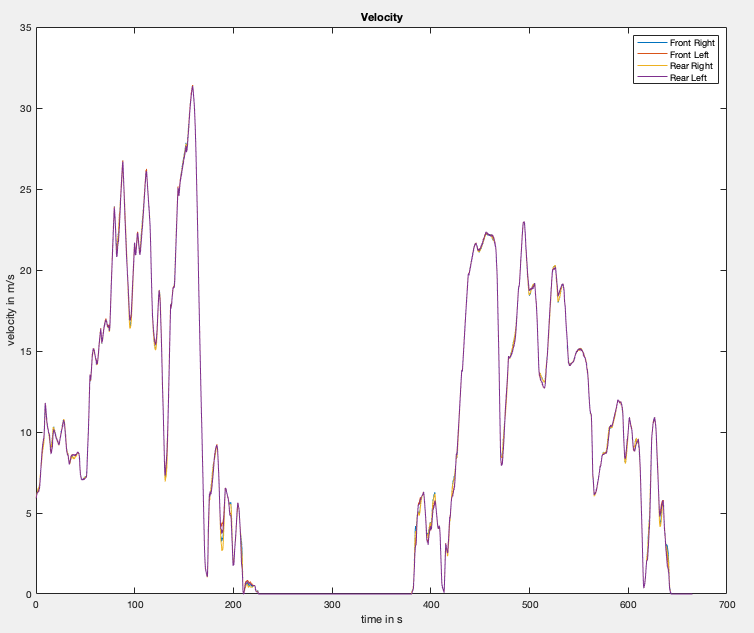
\includegraphics[width=1\linewidth]{../Graphiken/velo_ohneRand}
		\caption{Übersicht der Geschwindigkeiten der vier Räder}
		\label{fig:velo_ohneRand}
	\end{figure}
\pagebreak
%figure('NumberTitle','off','Name','Velocity')
%plot(tv,vfr);
%hold on;
%plot(tv,vfl);
%plot(tv,vrr);
%plot(tv,vrl);
%xlabel('velocity in m/s'); 
%ylabel('time in s');
%legend('Front Right', 'Front Left', 'Rear Right', 'Rear Left');
%title('Velocity');

	%\begin{figure}[h!]
	%	\centering
	%	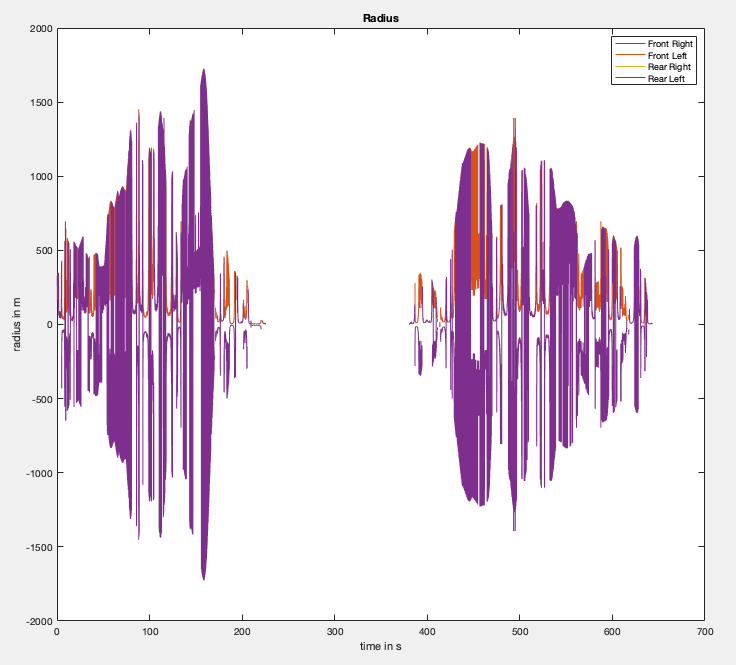
\includegraphics[width=1\linewidth]{../Graphiken/radius}
	%	\caption{Übersicht den Radius der vier Räder}
	%	\label{fig:radius}
	%\end{figure}
% %Alle Radien in einem Plot
% figure('NumberTitle','off','Name','Radius')
% plot(tv,rfr);
% title('Radius');
% hold on;
% plot(tv,rfl);
% plot(tv,rrr);
% plot(tv,rrl);
% xlabel('time in s');
% ylabel('radius in m')
% legend('Front Right', 'Front Left', 'Rear Right', 'Rear Left');

	Die \autoref{fig:velo_vs_sw} zeigt einen Ausschnitt zwischen 495s und 550s. Die Abbildung wurde in einzelne Abschnitte zur Analyse unterteilt. Im ersten Abschnitt, vor 500ms, ist der Lenkradwinkel sehr klein. Man sieht dort kaum keinen Unterschied zwischen den Geschwindigkeiten der linken und rechten Rädern. Im zweiten Abschnitt ist der Lenkwinkel wesentlich höher. Das hat zur Folge, dass die Geschwindigkeit der rechten Räder über der Geschwindigkeit der linken Räder liegt. Beim Wechel vom zweiten in den dritten Abschnitt ist der Winkel kurz Null und steigt dann wieder. Dort liegt die Geschwindigkeit der linken Räder über der Geschwindigkeit der rechten Räder. Daraus lässt sich schließen, dass sich die Fahrt von einer Links- in eine Rechtskurve ändert. Im vorletzen Abschnitt ist wieder eine Linkskurve erkennbar. Im letzten Abschnitt wird kaum gelenkt, aus diesem Grund weichen die Geschwindigkeiten nur sehr gering voneinander ab.
	\begin{figure}[h!]
		\centering
		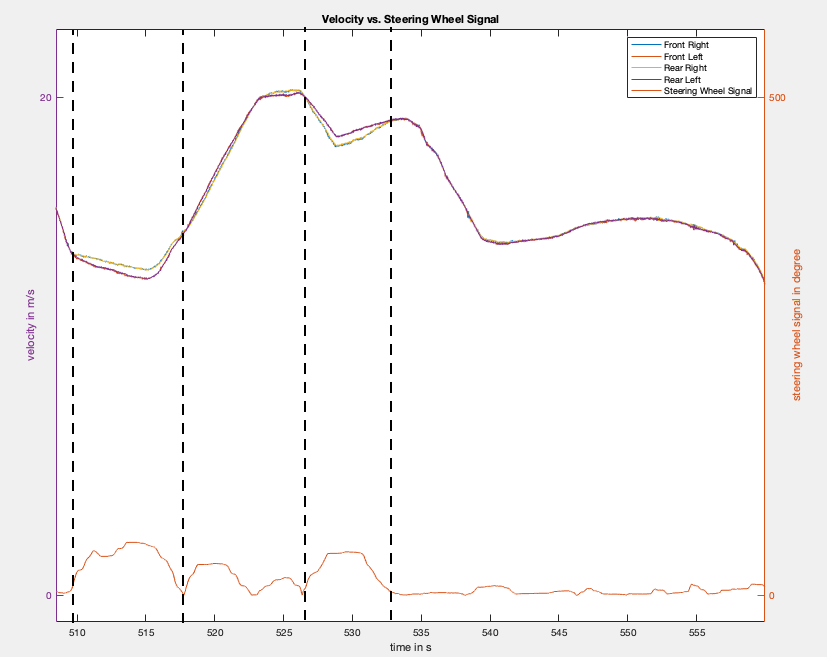
\includegraphics[width=1\linewidth]{../Graphiken/velo_vs_sw}
		\caption{Übersicht der Geschwindigkeiten mit Drehwinkel des Lenkrads}
		\label{fig:velo_vs_sw}
	\end{figure}
%%Alle Geschwindigkeiten in einem Plot
%figure('NumberTitle','off','Name','Velocity')
%plot(tv,vfr);
%hold on;
%plot(tv,vfl);
%plot(tv,vrr);
%[hAx,hLine1,hLine2] = plotyy(tv,vrl,tv,sw);
%xlabel('time in s'); 
%ylabel(hAx(1),'velocity in m/s');
%ylabel(hAx(2),'steering wheel signal in degree');
%legend('Front Right', 'Front Left', 'Rear Right', 'Rear Left', 'Steering Wheel Signal');
%title('Velocity vs. Steering Wheel Signal');
%für zusätzlichen Drehwinkel --> Links oder Rechtsfahrt
\newpage
	Die \autoref{fig:outter_vs_inner} zeigt den Ausschnitt von ca. 510ms bis 517ms. Dieser entspricht dem dem zweiten Abschnitt der \autoref{fig:velo_vs_sw}. Hier werden die Radien der beiden Vorderräder verglichen. Es ist erkennbar, dass der Radius des Rechten Vorderrads immer über dem Radius des Linken liegt. Dies zeigt nochmal, dass es sich hier um eine Linkskurve handelt.
	\begin{figure}[h!]
		\centering
		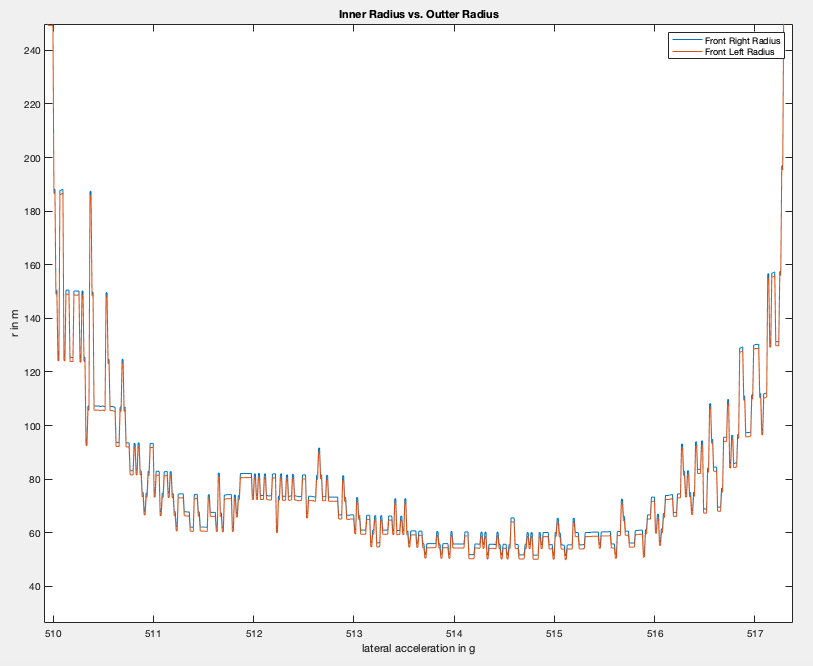
\includegraphics[width=1\linewidth]{../Graphiken/outter_vs_inner}
		\caption{Vergleich des linken und rechten Radius bei Kurvenfahrt}
		\label{fig:outter_vs_inner}
	\end{figure}
\cleardoublepage
\newpage
% %Vorderer Innerer Radius gegen Äußeren Radius
% figure('NumberTitle','off','Name','Inner Radius vs. Outter Radius')
% plot(tv,rfr);
% hold on;
% plot(tv,rfl);
% xlabel('lateral acceleration in g')
% ylabel('r in m');
% legend('Front Right Radius','Front Left Radius')
% title('Inner Radius vs. Outter Radius');


	In der nächsten \autoref{fig:sorted_sw} wird der Radius in Abhängigkeit des Drehwinkels abgebildet. Es zeigt, dass mit steigendem Drehwinkel der Radius immer kleiner wird. Stellen, an denen das Fahrzeug nicht fährt, können hierbei vernachlässigt werden. Allgemein gilt, dass bei Kurvenfahrten der Radradius abnimmt.
	
		\begin{figure}[h!]
		\centering
		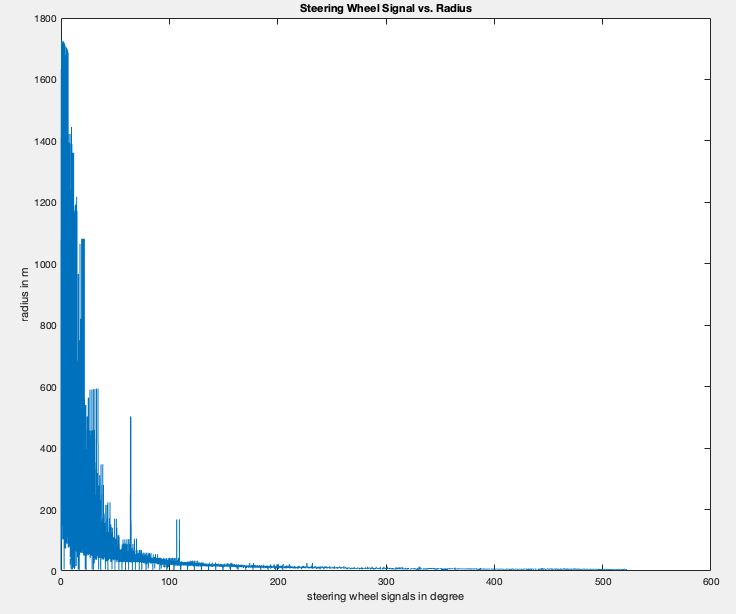
\includegraphics[width=1\linewidth]{../Graphiken/sorted_sw}
		\caption{Lenkraddrehwinkel gegenüber Radius}
		\label{fig:sorted_sw}
	\end{figure}
\pagebreak
% %Sortiertes sw gegen Radius
% figure('NumberTitle','off','Name','Steering Wheel Signal vs. Radius')
% plot(sw_sorted,newrfl);
% xlabel('steering wheel signals in degree');
% ylabel('radius in m');
% title('Steering Wheel Signal vs. Radius');
% %Sortiertes q gegen Radius
% [q_sorted, q_order] = sort(new_q);
% nrfl = rfl(q_order,:);
% figure('NumberTitle','off','Name','Sorted Lateral Acceleration vs. Radius')
% plot(q_sorted,nrfl);
% xlabel('sorted lateral acceleration in g');
% ylabel('radius in m');
% title('Sorted Lateral Acceleration vs. Radius');	

	In der folgenden \autoref{fig:v_vs_r} wird der Radius in Abhängigkeit der Geschwindigkeit dargestellt. Es zeigt, dass bei gleichem Drehwinkel des Lenkrads bei steigender Geschwindigkeit der Radius immer größer wird. 
	\begin{figure}[h!]
		\centering
		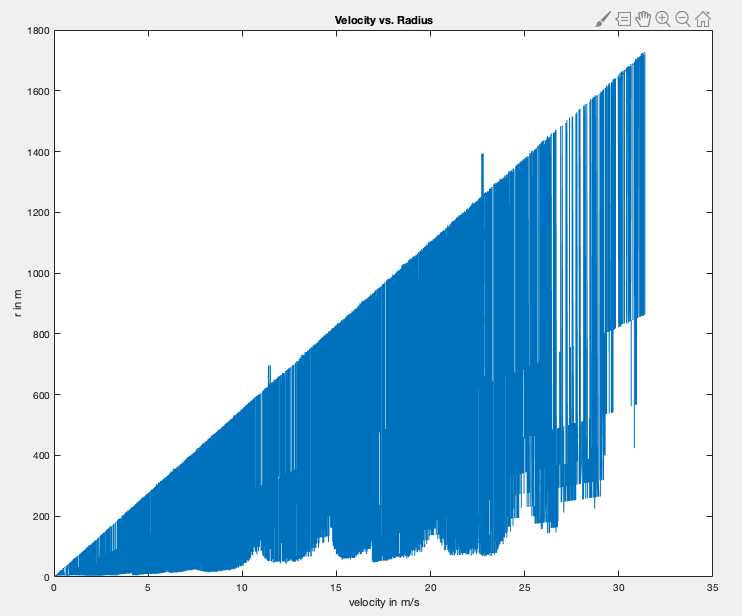
\includegraphics[width=1\linewidth]{../Graphiken/v_vs_r}
		\caption{Geschwindigkeit gegenüber Radius}
		\label{fig:v_vs_r}
	\end{figure}
% %Geschwindigkeit vs Radius SORTIERT
% [v_sorted, v_order] = sort(vfl);
% newradius= rfl(v_order,:);
% figure('NumberTitle','off','Name','Velocity vs. Radius')
% plot(v_sorted,newradius);
% %hold on;
% %plot(tv,rfl);
% xlabel('velocity in m/s')
% ylabel('r in m');
% %legend('Front Right Radius','Front Left Radius')
% title('Velocity vs. Radius');



	
	

	
	
	
	
	% Kapitel 2
	%Kaptitel 1

\chapter{Aufgabe D2}
\section{Section}
\subsection{SubSection}
\subsubsection{SubSubSection}
	

		
	% Abschlussbewertung
%	\input{content/Abschlussbewertung.tex}	
	
	% Glossar
%	\printglossaries %[style=altlist,title=\langglossar]
	
	% sonstiger Anhang
	\clearpage
%	\appendix
%	% !TeX root = ../dokumentation.tex

%\addchap{\langanhang}

%{\Large
%\begin{enumerate}[label=\Alph*.]
%	\item test
%\end{enumerate}
%}
%\pagebreak

%\section*{A. test}\label{sec:test}
%%\includegraphics[width=1\textwidth]{NameNodeWebInterface.png}
%\pagebreak



	
\end{document}
